% !TEX TS-program = pdflatex
% !TEX encoding = UTF-8 Unicode

% This is a simple template for a LaTeX document using the "article" class.
% See "book", "report", "letter" for other types of document.

\documentclass[11pt]{article} % use larger type; default would be 10pt

\usepackage[utf8]{inputenc} % set input encoding (not needed with XeLaTeX)

%%% Examples of Article customizations
% These packages are optional, depending whether you want the features they provide.
% See the LaTeX Companion or other references for full information.

%%% PAGE DIMENSIONS
\usepackage{geometry} % to change the page dimensions
\geometry{a4paper} % or letterpaper (US) or a5paper or....
% \geometry{margin=2in} % for example, change the margins to 2 inches all round
% \geometry{landscape} % set up the page for landscape
%   read geometry.pdf for detailed page layout information

\usepackage{graphicx} % support the \includegraphics command and options

% \usepackage[parfill]{parskip} % Activate to begin paragraphs with an empty line rather than an indent

%%% PACKAGES
\usepackage{booktabs} % for much better looking tables
\usepackage{array} % for better arrays (eg matrices) in maths
\usepackage{paralist} % very flexible & customisable lists (eg. enumerate/itemize, etc.)
\usepackage{verbatim} % adds environment for commenting out blocks of text & for better verbatim
\usepackage{subfig} % make it possible to include more than one captioned figure/table in a single float
\usepackage{graphicx}
\usepackage{float} 
% These packages are all incorporated in the memoir class to one degree or another...

%%% HEADERS & FOOTERS
\usepackage{fancyhdr} % This should be set AFTER setting up the page geometry
\pagestyle{fancy} % options: empty , plain , fancy
\renewcommand{\headrulewidth}{0pt} % customise the layout...
\lhead{}\chead{}\rhead{}
\lfoot{}\cfoot{\thepage}\rfoot{}

%%% SECTION TITLE APPEARANCE
\usepackage{sectsty}
\allsectionsfont{\sffamily\mdseries\upshape} % (See the fntguide.pdf for font help)
% (This matches ConTeXt defaults)

%%% ToC (table of contents) APPEARANCE
\usepackage[nottoc,notlof,notlot]{tocbibind} % Put the bibliography in the ToC
\usepackage[titles,subfigure]{tocloft} % Alter the style of the Table of Contents
\renewcommand{\cftsecfont}{\rmfamily\mdseries\upshape}
\renewcommand{\cftsecpagefont}{\rmfamily\mdseries\upshape} % No bold!

%%% END Article customizations

%%% The "real" document content comes below...

\title{Thesis Draft}

\author{Rubei Riccardo}
%\date{} % Activate to display a given date or no date (if empty),
         % otherwise the current date is printed 

\begin{document}
\maketitle
\newpage
\tableofcontents
\newpage




%Introduction
%% Mention CROSSMINER THe work has been done in that context...

%Mearuring the Similarty of SOftwre Systems
% %You can use some of the content from D6.2. Hopefully, CROSSSim can be included in this section as existing work (saying that it has been developed in the context of CROSSMINER

%Detailed description of the CLAN implementation

%Detailed description of the MUDABlue implementation

% Comparison CROSSSIM,CLAN and MUDABlue, RepoPal
%% Conduct evaluatin on the dataset f 580 Github projects


% Conclusion and Future Work








\section{Introduction}


\subsection{Overview}

A general introduction of Crossminer, my work and how it contributes.

\section{The Similarity Problem}

\subsection{Overview}

How to solve the problem of similarity between documents, subsection about SVD, LSI and other techniques.

\section{MUDABlue}

\subsection{Overview}

The first procedure analysed was MUDABlue, unfortunately none implentation was available on the web, so i reimplemented it from scratch. The MUDABlue method is an automatc categorizaton method or a large collecton of software systems. MUDABlue method does not only categorize sooware systemsd but also determines categories rom the sooware systems collecton automatcally. MUDABlue has three major aspects: 1) it relies on no other information than the source code, 2) it determines category sets automatically, and 3) it allows a software system to be a member of multiple categories. Since we were interested only in the evaluation of the similarity we discarded the phases related to clusterization and categorization.

\subsection{The Approach}

The MUDABlue approach can be briefly summarized in 7 steps, as the following image depicts:

\begin{figure}[H]
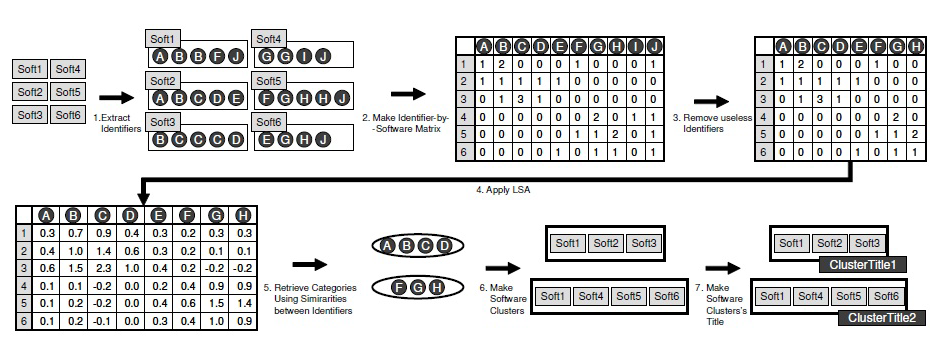
\includegraphics[width=15cm,height=20cm,keepaspectratio]{images/Mudablue1.png}
\centering
\caption{MUDABlue phases.}
\end{figure}

\subsubsection{Exctract Identifiers}
With identifier we are talking about relevant strings that can allow to characterize a document. In this phase each repository is scanned in order to find the target files, and for each of them the identifiers are exctracted, avoiding adding useless items such as comments. The dataset was a 41C projects gathered from SourceForge.

\subsubsection{Create identifier-by-software matrix}
As stated before, the main item to work with is the term-document matrix, in this case we count how many times each term appears in each file for all the projects. The result is matrix \textbf{m x n} with m terms and n projects.

\subsubsection{Remove useless identifiers}
From the matrix we remove all the useless terms, that is all the terms that apperas in just one repository, considered a specific terms, and all the terms that appears in more than 50\% of the repositories, considered as general terms.

\subsubsection{Apply the LSA}
Once the matrix is ready con be worked, the SVD procedure is applied and then the LSI. As explained before [NOTE] the SVD procedure decompose the original matrix in 3 other matrices. When we multiply back these matrices we use a rank reducted version of the S matrix in order to generete the final one. The authors didn't provide us any details about their final rank value, so we tested many values and eventually selected one.

\subsubsection{Apply the Cosine Similarity}
By using the cosine similarity method, we compare each repository vector with all the others and eventually getting an \textbf{n x n} matrix, in which is expressed the similarity of all the repository couple, with a value [0.0-1.0].

\subsubsection{Categorization}
The point 6 and 7 are not covered because not related to our work.

\section{Clan}

\subsection{Overview}

A description of Clan approach.

\section{Implementation}

\section{Results}

\section{Conclusion}

\end{document}
